\documentclass[sigconf]{acmart}
\usepackage{amsmath, amssymb, amsfonts}
\usepackage{amsthm}
\usepackage{algorithm}
\usepackage{algorithmic}
\usepackage{graphicx}
\usepackage{subfig}
\usepackage{xspace}
\usepackage{multirow}
\usepackage{rotating}
\graphicspath{{./graphs/}}

\renewcommand{\arraystretch}{1.3}
\newcommand{\tabincell}[2]{\begin{tabular}{@{}#1@{}}#2\end{tabular}}
\newcommand{\system}{SRAS \xspace}

\renewcommand \footnotetextcopyrightpermission[1]{}
\settopmatter{printacmref=false}

\begin{abstract}
    The return on investment (ROI) analysis about movies is a challenging but important task for movie investors in their decision making process. For investors, they are expected to get high box-office revenue with appropriate investments. Apart from movie special effects, most of investments are used to remuneration for movie actors(actress). Due to complicated factors such as audience reactions, screenplay, film types etc, it's not easy for investors to estimate upfront ROI, which makes film investment a gamble. Although most current research works aim to predict box-office revenue more specific, they can not provide investors more direct profits information about the success of the movie they would like to invest.
    \par In this paper, we design and implement an integreated system, called Social Network Investment Platform (a.k.a \system), that aims to do some analysis of movies for investors. \system provides various modules for users to predict box-office, capture public opinion about a film, assess the value of the actor, monitor the changes of the ratio of box-office about actors, assess actor replacement and so on.

\end{abstract}

\keywords{Data Analysis, Targeted Sentiment Analysis, Box-office Predicting}

\begin{document}

\title[SRAS: A  Social-respected Analysis System for Modern Movie Investment]{SRAS: A  Social-respected Analysis System for \\ Modern Movie Investment}

\maketitle

% ------------------------ intro -------------------
\section{INTRODUCTION}
\par In modern society, watching movies is becoming a central part of consumer culture which makes the great earning of investments about movies. However, how to evaluate the reasonability of investments becomes an important problem for investors. Owing to complex movie markets,  the success of a movie is closed related to audience reactions, screenplay, movie types and famous cast and directors.  Before a movie releases, we cannot guarantee it can be popular or not.
\par In recent years, with the heat of the movie market, large amounts of money pour into movie industry. Investments about movies consist of cast's and directors' salary,  movie itself production. advertising fees etc. Actors and directors salary occupies a large proportion in cost of movies. The immaturity of the Chinese film market itself leads to a high-risk, high-reward investment environment.Many investors determine the investment prospects of the film is based on the recent case of the same type of movie, but they do not have in the analysis of the case from the aspect of artistic creation (such as the type of film plot, actor and director of skill etc.) the ability to summarize experience of selling products, most will eventually reduced to the accumulation of the casting and some business element. This is a lot of investment some important reasons can be started the project and ultimately a huge loss.
\par Recently, the group acts of "fans" do not only create a great social effect, but also produce a huge economic benefit. Without bankable stars the film script aroused no interest. In order to pursue high profit, the usual way is to use a large number of "celebrities" to promote the box office through the fan effect but only a few were success. But it has caused the soaring star worth, the consequent increase in production costs. The reason is that in spite of massive "fans", the degree of match between fans and movies is the most important factor affecting the box office. Another is that box office is decided by actors, scripts, publicity, release schedule and other aspects, actors' contribution to the movie cannot be equal to box office. The lack of an effective quantitative method to assess the creative record of the box office contribution prevent investors from assess the investment star's rationality.
\par Besides the cost of production about movies, investors are concerned about box-office revenue. The research on movies maily focuses on movie box-office prediction\cite{marshall2013forecasting,basuroy2003critical,asur2010predicting}. They use linear regression, neural networks\cite{sharda2006predicting} and other models to predict box office more accurately by constructing multiple features, for instance, Google \cite{panaligan2013quantifying} uses search, ad click data, and line rows to predict box office and gets 94\% accuracy. Sentiment analysis in movie reviews \cite{manek2017aspect,kiritchenko2014sentiment,pang2008opinion} is another aspect to do some analysis in movies and many experiments\cite{gemser2007impact,joshi2010movie} prove that reviews data can improve box-office predicting accuracy.
\par In recent years, the research on movie mainly focuses on the construction of user-oriented movie recommendation system\cite{diao2014jointly,tang2015user}. However, those work are too simple to do some analysis on the components of revenue further. Generally speaking, investors are anxious to have a tool or a platform to do a more intuitive analysis of a movie's return on investment. In general, an investor-oriented movie analysis platform is for the Chinese movie market, providing an investor-oriented integrated emotional analysis, box office prediction, actor evaluation, box office contribution analysis of the analysis of the box office analysis of the movie, focusing on the protagonist, director, audience impact on the box office.
\subsection{Solutions and Challenges}
As methods developments in machine learning especially text mining increasing rapidly, much data mining techniques are proved to be effective method in both natural language process (NLP) and deep learning (DL). Social-respected analysis system(\system) is an end-to-end platform which aim to integrate social data of movies when analysing their investment value and potential future. \system makes great contribution in mining movie industry data from three points of view. We summarized it the actress played by actor, box-office pay back for investors, and sentiment reflect by audience. We proposed target-depend sentiment analysis for sentiment side, dynamic predition for box-office and finally the heteogenous network for investor. The key problem \system focused on are listed below.
\newtheorem{difficulties}[theorem]{difficulty}
\begin{difficulties}
Given a comment, how do you analyze the names and emotions mentioned in this comment? \end{difficulties}
\par The existing sentiment analysis of movie reviews rarely seldom further analyzes the sentiment of the commentators. In social media, audiences may show different affective tendencies toward different protagonists of the movie, where traditional short text sentiment analysis can not capture these sentiments. To solve this problem, \system provides an object-oriented commentary sentiment analysis that performs named entity recognition and sentiment classification for each comment to more accurately capture the viewer's preference for a particular director (actor) of a particular movie.
\begin{difficulties}
How to quantify the director's contribution to the box office?
\end{difficulties}
\par Director (starring) contribution to the box office refers to the audience for the expectations of one or a few people to generate consumer spending movie tickets, analyze the contribution of a box office contribution to help get the actual business director or director value. In the analysis of the box office data, it is difficult to quantify the actual box office revenue of every star / director in a movie. There is also a lack of analysis of related modules in the existing commercial movie analysis system.
\system provides a dynamic analysis module that accounts for the share of the box office's contribution, not only to quantify the box office's contribution but also to analyze the changes in the commercial value of a master before and after the release of the movie through changes in contributions over time.
\begin{difficulties} Joint value evaluation and replacability among actors.\end{difficulties}
\par Since effect of an actor suffer multi uncertainties and how to make a joint-evaluation of actor impact is a big question. A lot of method focus on giving linear weight for each factor. But this weight might change and impractical when goal of analysis changing. In \system, we mining joint value based on relationship among actors using heterogeneous network. Qualifying similarity and measuring increase of influence by co-star of two specific actor for target movie show great power on practicability of the system which enhance availability and effectiveness of \system a lot.
\begin{difficulties}
In which way the unstructured data cooperate with structured data?
\end{difficulties}
\par It is a  problem how much effect by just using reviews(the unstructured data) or combine many other factor in analysis. We see that integrate sentiment help to prediction and investment, considering textual data an intensifying factor for attribute of movie itself. Whether the effect existing in each other if we analyse the synergy effects is unknown. To solve this problem, constrained network and iterative algorithm have been proposed to capture effect between the two kinds of data.

\subsection{Roadmap}
The rest of this paper is organized as follows, Section \ref{sec:overviw} presents an overview of \system. In section \ref{sec:sent} we further study name entities recognition based on disambiguation and then describe how \system extract target-dependent sentiments and analyse changeable trend on sentiment. Section \ref{sec:impact} presents dynamic impact of leader creators based on both sentiments and self attributes. In section \ref{sec:predict} present the core value of system by phased prediction of movies which helps to maximum box-office based on reasonable investments now and future. Section \ref{sec:evo} presents system evaluation as well as the case study. In section \ref{sec:related}, we introduce the related work. Finally, Section \ref{sec:conclu} concludes the paper. 
% -------------------------platform--------------------
\section{Platform Overview}
\label{sec:overviw}
\begin{figure*}[!htbp]
  \centering
     \subfloat[dashboard]{%
  \includegraphics[width=2.0in]{screenshot5.png}}\hfill
    \subfloat[heterogeneous network]{%
  \includegraphics[width=2.0in]{screenshot1.png}}\hfill
    \subfloat[dynamic impact]{%
  \includegraphics[width=2.0in]{screenshot2.png}}\hfill
    \subfloat[phased box-office predicting]{%
  \includegraphics[width=2.0in]{screenshot3.png}}\hfill
%   \subfloat[film level sentiment]{%
%  \includegraphics[width=2.0in]{screenshot4.png}}\hfill
 
  \caption{Screenshots of FKAP}
\end{figure*}

\begin{figure}[!htbp]
\centering
\includegraphics[width=0.8\columnwidth]{overview.eps}
\caption{System architecture}
\label{fig:mhin}
\end{figure}

\system is a web-based integrated system for movie analysis. The screenshots of \system are shown in Figure 1 and the architecture overview is displayed in Figure 2. Using \system, users can carry out a series of analysis based on the movie centric information.
\par In general, \system consists of three layers of components, including Basic Processing Task Layer, Higher Algorithm Library Layer and Visualization Layer.
\par Basic Processing Task Layers provides data cleaning, data standardization and data conversion. Due to the different data sources, the data obtained can not be applied directly to the analysis. In fact, the movie data need to consider the following questions, name ambiguity elimination, used to evaluate the quality of the film at the box office, the film's reviews of object identification, actor knowledge base construction. These methods are provided in the basic processing task layer.
\par Higer Algorithm Library Layer contains the core technology of \system, including Target-Dependent Sentiment Analysis Module and Dynamic Impact of Actors and Directors Module. The layer considers the importance of film reviews to a film and combine with Machine Learning.
\par Visualization Layer is the interface between the system and the users. To intuitively present the analysis results, this layer is designed to be user-friendly and easy to operate. Specifically, Sentiment Tendency is ... 
% ------------------------ sentiment -------------------
\section{Practical Sentiment Analyse}
\label{sec:sent}
\par The main purpose of sentiment analyse is to discover views and opinions diversity of different targets in films which reflect what attract audience watching the movie. The sample dataset in this area are review corpus $ R =\{r_1, r_2, \dots, r_n\}$ and each $r_i$ has film name  $f_i$ it belonging to, time point $time_i$ , scores towards this film $s_i$ and user $u_i$ who scores. These attributes of reviews are discrete (has domain specific value) and many sentences in it contribute to the whole sentiment of this single review. Since reviews are spread in social media platform such as twitter or micro-blogs, the sentences are limited and review of movie are usually enough short. Thus, many phenomenon occurred on short texts or natural language add difficulties when analysing the sentiments of targets (e.g. Rhetoric, metaphor, proverb and nicknames). Unlike many works focus on proceed in sentence-level document-level and time-period level step by step, we try to figure out the sentiment to a specific actors or director(leading creator of this film). A useful prior knowledge in reviews together with reviewers' rating score or stars made by user is evaluation score of specific film. We make the best of this knowledge to enlarge our sentiment words database because user usually behave consistent sentiment to same target.

\subsection{Named Entities Recognition}
\par If we want to know sentiments behind human expression, targets that people are taking about should be identified firstly. Here we concentrate on comment target about leader creators in films. The main challenging is the nicknames for actors and directors.
\par \textbf{Sequence to sequence approach}. Given a word sequence $X=\{x_1, x_2, \dots, x_n\}$ we observed and the 4-tag label set $Tags=\{O,B,E,M\}$, the objective task is to find correct corresponding labels $Y=\{y_1, y_2, \dots, y_n | y_i \in Tags\} $. By optimizing the loss function with parameter $ \theta $
\begin{equation}
    J(\theta)= \arg\min_{\theta} \frac{1}{n}\sum_{i=1}^{n}loss(f(x_i;\theta), y_i)
\end{equation}
recurrent neutral networks such as \emph{LSTM}, \emph{BidirectionalLSTM}, \emph{BidirectionalLSTM+CRF} have been proved to be state-of-art structures. They consider both long time and short terms information and find tags with maximum possibility for sequence labeling. However, previous machine learning approaches need huge domain training data, while it is hardly to label these social media corpus accurately which are full of informality and flexibility. Especially actors get constantly evolving new roles in various films as time goes by, we hope find a simple and efficient way that recognize most of the comment targets in films reviews.
\par \textbf{Fast and adaptive approach}. In order to mining entities in linear time, we apply key word matching for leader creators in films. Online knowledge database which store film meta information can be strong support providing comprehensive and dependable analysis. Focused crawling technology based on web linkage contribute to construction of prior knowledge of \textbf{actors}, \textbf{roles} and \textbf{directors}.

\begin{algorithm}[htb]
\renewcommand{\algorithmicrequire}{\textbf{Input:}}
\renewcommand\algorithmicensure {\textbf{Output:} }
\caption{ Framework of nickname mining for our system}

\begin{algorithmic}[1]

\REQUIRE ~~\\
The name set of \textbf{actors} and \textbf{directors} in each film\\
The name set of \textbf{roles} for each actors used to played\\
Threshold $\boldsymbol\alpha$ for minim similarity of misspell and variation\\
Threshold $\boldsymbol\beta$ for max tolerance of misspell and variation\\

\ENSURE ~~\\
Potential comment targets mapping dictionary $A$, $P$\\

\STATE Aggregating reviews group by corresponding film name along with preparing actors list $A_i$, directors list $P_i$ in $i$th film according given \textbf{actors} and \textbf{directors};
\STATE Constructing actors mapping $A$ for every actor in $ a_i$, so dose $P$ for every director in $p_i$;
\STATE Quality similarity between every noun morphemes $w$ and $t$ in \textbf{roles}, \textbf{actors} and \textbf{directors} by \emph{Jaccard} char distance in all comments for one film;
\STATE Recognizing potential nickname by the similarity and threshold $\boldsymbol\alpha$ we set, if $Jaccard(w, t) > \alpha$ add it to mapping dictionary $A$ or $P$;
\STATE Checking potential nickname in mapping dictionary, if $Levenshtein(w, t) > \beta $, delete it from mapping dictionary $A$ or $P$;
\RETURN $A$, $P$

\end{algorithmic}
\label{alg:ner}
\end{algorithm}

\begin{table*}[!t]
\begin{center}
  \centering
  \begin{tabular}{|c|c|c|c|c|c|c|}
    \hline
    Review No. & Contents & Referred & Film No.& time point  & Scores \\
    \hline
    1 & \tabincell{l}{Yang Yang's hard temperament\\ is enough to hold up the role} & Yang Yang & Ten great II of peach blossom & 2016-07-25T13:36:12.000+0800 & 10\\
    2 & \tabincell{l}{Yang Yang's acting is really \\ embarrassing, Crystal Liu is OK} & \tabincell{l}{Yang Yang,\\ Crystal Liu}& Ten great II of peach blossom & 2017-08-07T20:18:55.000+0800 & 5\\
    3 & \tabincell{l}{The story of embarrassment,\\ feeling Yehua did not love Baiqian} & \tabincell{l}{Yang Yang,\\ Crystal Liu} &  Ten great II of peach blossom & 2017-08-07T21:09:07.000+0800 & 2\\
    $r_i$ & \dots & \dots & $f_i$ & $time_i$  & $s_i$ \\
    \hline
  \end{tabular}
  \caption{review targets after named entities recognition}
\end{center}
\label{tab:summary}
\end{table*}

\par Assume average noun morphemes length is $m$ for all $n$ reviews and $t$ targets for all $F$ films. Algorithm \ref{alg:ner} need compare $ c \times nmt$ times. Since word comparing consume limited space and time and $ m \ll n, t \ll n $, we extract potential comment targets in $ O(n) $ time complexity which greatly less than deep learning approach. We can easily adjust designed parameter and improve efficiency with parallel framework when processing TB data.

\par In order to decrease the storage space of data, we replace film name and user name by mapping them using film id and user id. $f_i \in F=\{f_1, f_2, \dots, f_m\}$ and $u_i \in U = \{u_1, u_2, \dots, u_U\}$. Let score for each review be $s_i \in [0, 10]$ and $time_i$ be the timestamps. The features we finally retrieved can be summarized in table \ref{tab:summary}.

\subsection{Target-Dependent Sentiment Classification}
\par Sentences tend to be more complex when targets we want to analyse increase and sentiments detection being a hard work when analysing more objects. We take leader creator of film as major targets in this paper. Examples containing multi targets are shown as follows.
\begin{enumerate}
  \item Live here now! The point of life is looking for the point. ---\emph{A dog's purpose}
  \item It has been a year since I were familiar with Alexander Sandro Gonzalez Inarritu whose films have a cruel irony and full bitterness.---\emph{Bird man}
  \item Mia had dreamed of becoming an actress known by more audience, while Sebastian want to won a place in his loving jazz. ---\emph{LaLa land}
\end{enumerate}
\par  Sentence(1) is a non-target review, while Sentence(2) shows one-target sample and Sentence(3) stands for multi-target sentences. Considering targets after NER process in section 4.1 consist of actors map list $A=\{a_1, a_2, \dots, a_A\}$ and directors map list $P=\{p_1, p_2, \dots, p_P\}$, we cluster sentences into comments set with two polarity(positive $+1$ and negative $-1$). Binary sentiment classifier play an important role in sentiment classification. Sentiment polarity $SP=\{+1, -1\}$ labeled by classifier for each sentences in corpus $st_i^j$ of $i$th film with corresponding target $j$, $j \in A \cup P $ and targets capacity $T = ||A||+||P||$. Let $T_i$ be number of targets in film $i$. We try to find out following segments.

\begin{equation}
    Neg=\bigcup_1^{F} ng_i \ | \ polarity \ of \ ng_i = -1, \ ng_i \in \bigcup_{j=1}^{T_i} st_i^j
    \label{eq:neg}
\end{equation}
\begin{equation}
    Pos=\bigcup_1^{F} ps_i \ | \ polarity \ of \ ps_i = +1, \ ps_i \in \bigcup_{j=1}^{T_i} st_i^j
    \label{eq:pos}
\end{equation}

\par Since we have to retrieve \emph{Neg} and \emph{Pos} shown in Equation (\ref{eq:neg}) and (\ref{eq:pos}), we take training data $R_p$ with scores larger than 9 for positive sentiment and $R_n$ which scores lower than 3 for negative one. We exclude reviews $R_{ambi}$ which scores range between 4 and 8 that might be ambiguous over sentiment in training phrase. Instead, $R_p$ and $R_n$ show more concentrated sentiments in words. We train a classifier on $R_p$ and $R_n$, then we split $R$ with context window according referred target in each review. Reviews segments cover target's contextual information which construct sentiment corpus $Neg$ and $Pos$ towards specific targets are objectives for sentiment classifier. We mainly apply it on targets segments split from $R_{ambi}$. Finally, we get comprehensive sentiment polarity on targets segments in $R$.

\par Lexicon based sentiment analysis is constrained by sentence structure, latent word meaning and confused word features. We introduce bidirectional long short term memory (\emph{Bi-LSTM}) neural network for end-to-end sentiment classification and automated feature learning as figure \ref{fig:lstm} shows.

\begin{figure}[!htbp]
\centering
\includegraphics[width=\columnwidth]{bi-lstm.eps}
\caption{Structure of Bi-LSTM Sentiment Classifier, where $L_r$ for target words length and $L_w$ for context length we extract from original sentence. First layer in Bi-LSTM stands for forward hidden layer and the second layer are the backward one.}
\label{fig:lstm}
\end{figure}

\par Specially, word sequence are represented as a low dimensional , continuous and valued vector. It is called word embedding and we use pre-trained vectors so as to make better use of semantic and grammatical associations. Assume each $d$-dimension vector $ W_i = \mathbb{R}^{d \times |V|}$ for $i$th word in whole vocabulary $V$. Targets words with $L_r$ length cover $tw = \{W_r, W_{r+1}, \dots, W_{r+L_r-1}\}$ and context words $cw = \{W_{r-L_w}, \dots, W_{r-1}, W_{r+L_r}, \dots, W_{r+L_r+L_w-1}\}$ with window length $L_w$ surround corresponding targets words $tw$. \emph{BiLSTM} maps word vectors to fix-length sentence vector by recursively transformation above vectors of previous time step $h_{t-1}$. Cells for \emph{BiLSTM} in Figure \ref{fig:lstm} contains neural gates: input gates, forget gates, and output gates which adaptively remember input vector, forget history, and generate output vector. We add softmax layer to output sentiment of sentence vector which cover hidden representation of vectors for specific target segment as Figure 1 shows. Core calculation in LSTM cells are listed in bellow equations. $\odot$ is element-wise multiplication and $\sigma$ is sigmoid activation, $W_i, W_f, W_o, b_i, b_f, b_o$ are parameters for input, forget and output gates.
\begin{subequations}
\begin{align}
  i_t &= \sigma(W_i \bullet [h_{t-1};w_t] + b_i)\\
  f_t &= \sigma(W_f \bullet [h_{t-1};w_t] + b_f)\\
  o_t &= \sigma(W_o \bullet [h_{t-1};w_t] + b_o)\\
  g_t &= \tanh(W_r \bullet [h_{t-1};w_t] + b_r)\\
  c_t &= i_t \odot g_t + f_t \odot c_{t-1}\\
  h_t &= o_t \odot \tanh(c_t)
\end{align}
\end{subequations}


\subsection{Film-level Sentiment Trend}
\par In this section, we mainly care about how to predict latent sentiment transform. Obviously, we quantify explicit sentiment towards special actors or directors. Although all information came from overall corpus, we can not deny that different sentiment exist in different time period during movie life. Audience's sentiments have trends and always behave dynamically. Previous work concentrate on sentiment polarity and we extend it by capture dynamic time-period sentiment. Denote a time period range from $time_r = [time_i, time_j]$, we capture review statistical sum $R_{f_i}$ of each movie $f_i$ at time period $time_r$ from $Pos$ and $Neg$. Then we get different target $j$'s positive or negative sentiment transformation at different $time_r$.

\begin{equation}
    SentimentPos^j_i (time_r) = 10\cdot \frac{|pos^j_i \ in \ time_r|}{R_{f_i}}
\end{equation}

\begin{equation}
    SentimentNeg^j_i (time_r) = 10\cdot \frac{|neg^j_i \ in \ time_r|}{R_{f_i}}
\end{equation}

\par Dynamic sentiment on leader creator shows how people transform their attention from different targets in movies. We pick out most interesting part (actor) from them and label it the main factor which mainly contribute to the box-office of specific film. The trend analyse is shown in Figure \ref{fig:sentiment}.

\par To measure the smoothness of the sentiment time series, we use slice window to capture the changes in the emotional inclination of the reviews. We Denote upper bound and lower bound of a day $r$,$UBP^j_i (r)$, $LBP^j_i (r)$,$UBL^j_i (r)$ and $LBN^j_i (r)$. 

\begin{equation}
    UBP^j_i (r) = mean^j_i (time_r)+\lambda \cdot std^j_i (time_r)
\end{equation}

\begin{equation}
    LBP^j_i (r) = mean^j_i (time_r)-\lambda \cdot std^j_i (time_r)
\end{equation}

where 
\begin{equation}
    mean^j_i (r) = \frac{1}{2d}\sum_{k=r-d}^{r+d}SentimentPos^j_i (time_k)
\end{equation}

\begin{equation}
    std^j_i (r) = \frac{1}{2d}\sum_{k=r-d}^{r+d}(SentimentPos^j_i (time_k)- mean^j_i (time_r))^2
\end{equation}

\par Because the time series follows Gaussian Distribution, and we set $\lambda=2$, means that confidence intervals is 0.0456, 

\begin{figure}[!htbp]
\centering
\subfloat[Period Sentiment Trend: Change of sentiment in a specific film]{\includegraphics[width=\columnwidth]{sentiment_1.eps}}
\hfill
\subfloat[Dynamic Sentiment on Leader Creator : General sentiment transform of an actor in past five years]{\includegraphics[width=\columnwidth]{sentiment_2.eps}}
\caption{Film-level sentiment trend analyse of different time period. a) shows the change of sentiment in one film life period which indicates what attract people. b) shows the average sentiment of a specific actor which indicates highest moments and lowest moment of an actor career }
\label{fig:sentiment}
\end{figure}



% ------------------------ impact -------------------
\section{Dynamic Impact of actors and directors}
\label{sec:impact}
The goal of this module is to find who is the most bankable person in a movie and to capture the dynamic trends about actors and directors during the period of a movie released.\\

\subsection{Contribution of Actors}
\begin{figure}[!htbp]
\centering
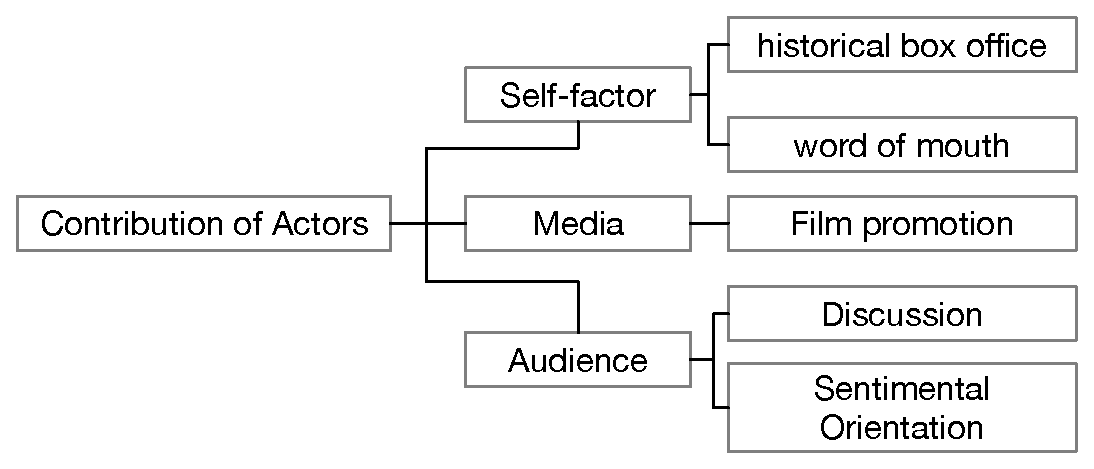
\includegraphics[width=0.8\columnwidth]{impact.eps}
\caption{Composition of creative influence}
\label{fig:mhin}
\end{figure}
The actor's own box office appeal. Actor's own box office appeal includes historical box office results and historical word of mouth performance, in which the film's historical movie box office performance can objectively reflect the creative ability of gold absorption, while the historical reputation score can objectively reflect the creative performance by Audience recognition, so this article at the same time using the history of the box office and the history of reputation to measure the creative box office call ability.\\
We define the The box office quality $boq$ to measure the box office generated by the creator itself based on the historical film data. As for directors, we define $boq=wms\cdot bos$.Considering different role importance, as for actors, we define $boq_k = c_k\dot wms\dot bos$, where $k$ is the $k$th actor and $c_k$ is the influence factor. The larger $k$ is , the smaller $c_k$ gets.\\
Media exposure. The movie's promotional period is always accompanied by a wide range of media coverage, the media's title content reflects the current public focus, if an actor or director appear in the title a lot, you can explain the public Familiarity and attention more.\\
Feedback from the audience. Liu mentioned the impact of word-of-mouth on the box office is very large (Liu, Y. (2006). Word of mouth for movies: Its dynamics and impact on box office revenue. Journal of marketing, 70 (3)). With the rapid development of the Internet, people can express their emotions on social media at any time. Thanks to the development of social media networks, the promotion of the movie has also gradually increased the proportion of online publicity. At the same time, the content of the discussion of the movie has also formed a considerable amount of data. The movie review often includes the concept of " If you can get the audience's idea of ​​an actor or master from the commentary, you can see whether the source of the audience's emotional inclination toward the movie comes from the influence of the movie's main actor (including the protagonist).\\
\subsection{Dynamic Impact of Leader Creator}
In the short life of the movie, the contribution of the genre to the box office is obviously not constant. With the development of the Internet media, real-time feedback of the movie users on the movie will affect the watching desire of the non-movie users, and the positive contribution Refers to the potential box office or the desire to watch the increase; the negative is the box office to bring the negative image, to dispel the wishes of watching. Therefore, in the film's life, the star effect on the box office's contribution is dynamic, the project will be divided into the life of the movie before the release, the first week of release, the second week of release, the third week of release, released the fourth Friday A period, respectively, to explore the five periods of major box office contributions. 
% ------------------------ hin -------------------
\section{Mining Movie Heterogeneous Network}
\par In order to discover important relation and promotion between two actors, we focus on mining movie heterogeneous information network. Discovering interesting topology of network provide great insight about the system innate character. A movie heterogeneous information network (\emph{MHIN}) is a domain information network with multiple types of entities and relations. We construct our \emph{MHIN} with multiple objects such as movies (M), directors (D), users (U), Actors (A), Types (T) and box-offices (B). Figure \ref{fig:mhin} shows typical \emph{MHIN} schema defined by us. Links exist between users and movies denoting score and score-by relations, between movies and actors(directors) denoting star(direct) and star-by(direct-by) relations, between movies and types denoting label and (labeled) relations, between movies and box-offices denoting gain and gain by relations. Also, we can add other attributes into the movie heterogeneous network (e.g years (Y), producers (P)). Meta-path is a connect relation between two types of objects in \emph{MHIN}. Denote network schema for our \emph{MHIN} is $\mathcal{S}=(\mathcal{A}, \mathcal{R})$, where $\mathcal{A}$ represent object types and $\mathcal{R}$ indicate different types of relationships. A meta-path $\mathcal{P}$ is defined in the form of $A_1 \xrightarrow{R_1} A_2\xrightarrow{R_2} \dots\xrightarrow{R_k} A_{k+1}$. Length of $\mathcal{P}$ is defined by number of relations it contains. Semantic composite relations are implied in meta-paths. For example, we can evaluate the similarity of movies or actors by length-2 meta-path MDM (movie-director-movie), MAM (movie-actor-movie) or AMA (actor-movie-actor), AMTMA(actor-movie-type-movie-actor).

\begin{figure}[!htbp]
\centering
\subfloat[Structure of movie heterogeneous network]{\includegraphics[width=0.8\columnwidth]{mhin.eps}}
\caption{Social network schema of MHIN.}
\label{fig:mhin}
\end{figure}

\subsection{Rank Based Cluster For Actors}
In this section, we introduce a way to make distinguish between A-list and B-list actors. We prefer applying cluster based classifier on actors popularity recognition. Strong available mutually reinforcing relations between cluster and rank are helpful to deal with different levels of actors. We defined recursion formula by following empirical rules.
\newtheorem{rules}[theorem]{rule}
\begin{rules} high rank actors star more high rank movies\end{rules}
\begin{rules} high rank movies attract more high rank actors\end{rules}
\begin{rules} actors get high rank with high rank co-starers\end{rules}

Suppose we want $K$ clusters of actors. According the star relationship between actors and movies, we define matrix $M_{MA}(i, j)=c_{ij}$ representing actor $j$'s contribution of movie $i$ (see Section 3.1) and similarly, $M_{AA}(i, j)= m_{ij}$ stands for number of movies that actor $i$ and actor $j$ co-stared. Note that $W_{AM} = W_{MA}^T$, and $i=\{1,2,\dots, m\}, j=\{1,2,\dots, n\}$. According the 3 rules we proposed, we have

\begin{subequations}
\begin{align}
  r_{A}(i) = \alpha \sum_{i=1}^{m}W_{AM}&(j, i)r_M(i) + (1-\alpha)\sum_{j=1}^{n}W_{AA}(i, j)r_A(j)\\
  r_{A}(j) &\leftarrow \frac{r_{A}(j)}{\sum_{j'=1}^{n}r_{A}(j')}\\
  r_{M}(i) &= \sum_{j=1}^{n}W_{MA}(i, j)r_A(j)\\
  r_{M}(i) &\leftarrow \frac{r_{M}(i)}{\sum_{i'=1}^{m}r_{M}(i')}
\end{align}
\end{subequations}

Note that $\alpha \in [0,1]$ is a believe factor of weighed component of rule 3,  $r_{A}(j)$ and $r_{M}(i)$ are normalized rank score vector. We finally get $r_A$ which should be primary eigenvector of $\alpha W_{AM}W_{MA} + (1-\alpha) W_{AA}$. Further, we capture posterior probability $\pi_{i,k}$ that $a_i$ from cluster $k$, Once an actor acts a movie, he is more likely to star high ranked film and for movie, its success are more likely contributed by high rank actor. Thus we have K dimensional vector $s_{a_i} = \{\pi_{i,1}, \pi_{i,2}, \dots, \pi_{i,K}\}$ where $\pi_{i,k}$ denotes $a_i$'s coefficient for component $k$.

The cluster center and the distance between each actor and each cluster can be defined as
\begin{subequations}
\begin{align}
  S_{A_k} &= \frac{\sum_{a \in A}s(a)}{|A_k|} \\
  Distance(a, A_k) &= 1-\cos(s_{a_i}, S_{A_k})
\end{align}
\end{subequations}

\begin{algorithm}[htb]
\renewcommand{\algorithmicrequire}{\textbf{Input:}}
\renewcommand\algorithmicensure {\textbf{Output:} }
\caption{RankClus for Actors}

\begin{algorithmic}[1]

\REQUIRE ~~\\
Our movie information network $MHIN=(M, A; W)$\\
Cluster Number $K$\\

\ENSURE ~~\\
$K$ clusters of actors $A_i$ and rank of actor in each cluster \\
\STATE iter = 0;
\STATE Init partitions for A, get $PA^{iter}=\{A_i^{iter}\}_1^K$;
\STATE Repeat following until $PA^{iter}-PA^{iter-1}<\epsilon$ or iterations reach limitation
\STATE \quad For all cluster calculate $r_A$ followed by rank function
\STATE \quad Evaluate $\Theta$ for mixture model and get component efficient estimations $s_{a_i}$ for each actor $a_i$
\STATE \quad Update centers $S_{A_k}^{iter}$ of each cluster $A_k$
\STATE \quad Reassign each actor $a_i$ according distance between $a_i$ and each cluster center $A_k^{iter}$
\end{algorithmic}
\end{algorithm}


\subsection{Alternative Actors}
In this section, we discuss method choosing alternative actors for casting agents. The basic idea is measure similarity between actors. Since movie information network has been built, we then introduce meta path-based similarity framework for alternative actors. The example is show in table \ref{tab:metapath}.

\begin{table}[!htb]
  \centering
  \begin{tabular}{c|c|c}
  \hline
  Type & Path instance & Meta-path \\
  \hline
  I(\emph{AMA})& Andy-$M_1$-Sara & \tabincell{c}{Actor-\\Movie-Actor}  \\
  \hline
  II(\emph{AMTMA}) & \tabincell{c}{John-$M_2$-Comedy-$M_3$-Sara\\Ben-$M_4$-War-$M_3$-Sara\\Drew-$M_5$-Dracula-$M_2$-John} & \tabincell{c}{Actor-Movie-\\Type-Movie\\-Actor} \\
  \hline
  III(\emph{AMDMA}) & \tabincell{c}{Diana-$M_6$-Spielberg-$M_1$-Andy\\John-$M_2$-Luc Besson-$M_5$-Drew\\Sara-$M_3$-Tom Tykwer-$M_5$-Drew} & \tabincell{c}{Actor-Movie-\\Director-Movie\\-Actor}\\
  \hline
  \end{tabular}
  \caption{Different Types of meta-path in MHIN}
  \label{tab:metapath}
\end{table}

Denote actors $a_1$ and $a_2$ then $p_{a_1 \rightsquigarrow a_2}$ is a path instance between $a_1$ and $a_2$, $p_{a_1 \rightsquigarrow a_1}$ is a path instance between $a_1$ and $a_1$, $p_{a_2 \rightsquigarrow a_2}$ is a path instance between $a_2$ and $a_2$. We then get similarity between $a_1$ and $a_2$ by calculate

\begin{equation}
  s(a_1,a_2) = \frac{2 \times |\left\{p_{a_1 \rightsquigarrow a_2}: p_{a_1 \rightsquigarrow a_2} \in \mathcal{P} \right\}|}{|\left\{p_{a_1 \rightsquigarrow a_1}: p_{a_1 \rightsquigarrow a_1} \in \mathcal{P} \right\}| + |\left\{p_{a_2 \rightsquigarrow a_2}: p_{a_2 \rightsquigarrow a_2} \in \mathcal{P} \right\}|}
\end{equation}

Base on this measure of actors, we can not only know similarities but also get multi metrics that reflect how actors link with others. Query a specific actor $a_i$and then return a recommend actor list $r_{a_i}$ that ordered by similarities. Investors can determine the scope of film plan or prepare backup candidate for chief actor. In \system we also analyse different types of meta path instances for providing comprehensive alternative information for other actors.

% ------------------------ case -------------------
\section{System Evaluation And Case Study}
\label{sec:evo}
% --------------- related work and so on-----------------
\section{Related Work}
\label{sec:related}

\section{Conclusion}
\label{sec:conclu}

\section{Acknowledgements}

% --------------- biblio ---------------
\bibliographystyle{ACM-Reference-Format}
\bibliography{SRAS}
\end{document} 